\chapter{Анализ предметной области} \label{ch1}
В данной главе рассматривается предметная область и описываются основные понятия, которые с ней связаны, представлены требования к разрабатываемому программному средству, а также постановка цели и задач выпускной работы.
\section{Описание предметной области, обоснование актуальности} \label{ch1:sec1}

На текущий момент компьютерная индустрия стремительно развивается, и это неразрывно связано с увеличением количества используемых программных продуктов и увеличением их сложности. В последние годы объем программного кода многих продуктов составляет миллионы строк.
С ошибками в программном коде сталкивался каждый программист и именно по этой причине на данный момент актуальна задача поиска этих ошибок.
Для поиска ошибок используются различные методики. Они могут быть как основаны на анализе только исходных кодов (методы статического анализа), так и на использовании информации времени выполнения (методы динамического анализа).
Динамические методы (такие как тестирование) просты в реализации, не требуют больших вычислительных затрат, но при этом позволяют выявлять ошибки только для конкретных трасс исполнения программы. 
Методы статического анализа характеризуются высокой вычислительной сложностью, но при этом позволяют обнаруживать ошибки во всех возможных трассах исполнения.\\

\begin{figure}[h]
	\center
	
\includegraphics [scale=1] {my_folder/images/my/1}
	\caption{Общая схема статического анализа} 
	\label{fig:1}  
\end{figure}

Модели программ делятся на структурные, поведенческие и гибридные. Структурные модели основаны на синтаксисе исходного языка, а поведенческие дополнительно используют семантику конструкций языков программирования.
К структурным моделям относят:
\begin{itemize}
\item Дерево разбора 
\item Абстрактное синтаксическое дерево\\
К поведенческим моделям относят:
\item Граф потока управления 
\item Статическое однократное присваивание
\item Граф зависимостей по данным
\item Граф зависимости программы
\end{itemize}
	К гибридным моделям относят абстрактный семантический граф.
\section{Описание моделей программ} \label{ch1:sec2}
Каждая из перечисленных моделей имеет свою область применения, связанную с целью проведения разбора (компиляция, оптимизация, распараллеливание, анализ и т. п.). Рассмотрим каждую из вышеупомянутых моделей подробнее и проведем анализ.
\subsection{Абстрактное синтаксическое дерево} \label{ch1:subsec-title-abbr}
Абстрактное синтаксическое дерево (Abstract Syntax Tree, AST) - дерево, которое в абстрактном виде представляет структуру программы. AST создаётся парсером по мере синтаксического разбора программы, обрабатывается путём обхода при проверке семантических правил и проверке/определении типов, а затем, также, путём обхода AST, выполняется генерация кода. В современных компиляторах AST и список диагностик (ошибок, предупреждений) — это два результата вызова модуля синтаксического разбора.
Данное дерево содержит полную синтаксическую модель программы без лишних деталей (таких, как пробельные символы или комментарии). Ниже представлен программный код и представлена визуализация AST. Данный код используется для всех последующих примеров в этой главе.

\lstset{
numbersep = 5pt,
stepnumber = 1
}

\begin{flushright}
Листинг 1.1. Метод sumOdd
\end{flushright}

\begin{lstlisting}
int sumOdd(int n) {
int s = 0;
int i = 1;
while (i <= n) {
	if (i % 2 == 1) {
		s += i;
	}
i++;
}
return s;
}
\end{lstlisting}


\newpage
\begin{figure}[h]
	\center
	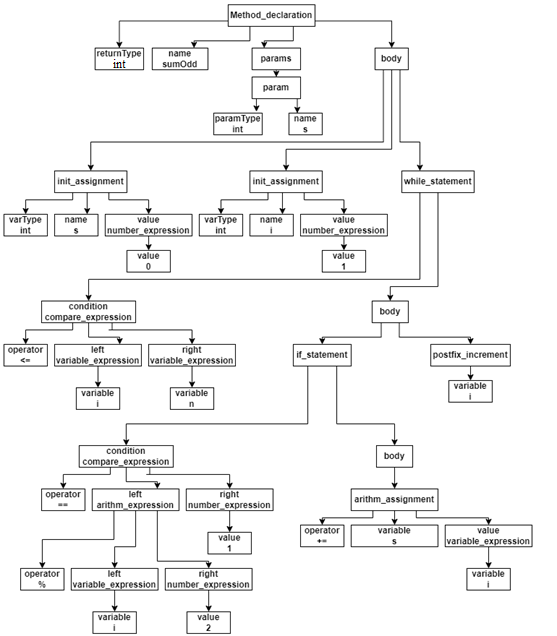
\includegraphics [scale=1] {my_folder/images/my/2}
	\caption{AST}
	\label{fig:2}  
\end{figure}

%\section{Граф потока управления} \label{ch1:sec2-abbr2}
\subsection{Граф потока управления} \label{ch1:subsec-title-abbr}
Граф потока управления (Control Flow Graph, CFG) — модель программы, представляющая в виде ориентированного графа поток управления в программе. В этой модели сохраняются только инструкции программы, а также информация о возможной передаче управления между инструкциями.
Каждый узел (вершина) графа соответствует базовому блоку - прямолинейному участку кода, не содержащего в себе ни операций передачи управления, ни точек, на которое управление передается из других частей программы. Имеется лишь 2 исключения: точка, на которую выполняется переход, является первой инструкцией в базовом блоке, и базовый блок завершается инструкцией перехода. Направленные дуги используются в графе для представления инструкций перехода. Достижимость — одно из свойств графа, используемое при оптимизациях. Если блок или подграф не имеют путей до них от входного блока, то данная часть графа является недостижимой (мертвый код) при любых вариантах исполнения, и по этой причине он может быть удален из программы. Если же из данного подграфа нет путей до выходного блока, то значит этот подграф содержит бесконечный цикл.
Граф потока управления используется для:
\begin{itemize}
\item Генерации кода 
\item Оптимизации программ 
\item Обнаружения ошибок в программе 
\item И т. п.
\end{itemize}

На рис. 1.3 изображен пример визуализации CFG.
\begin{figure}[h]
	\center
	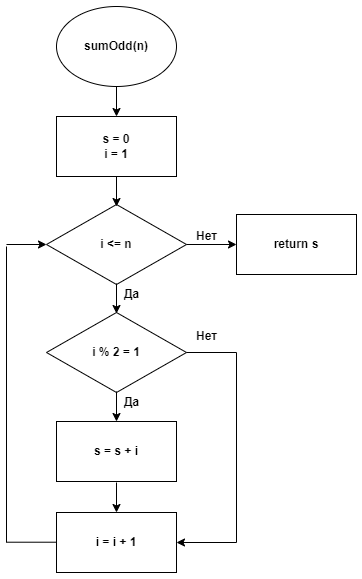
\includegraphics [scale=0.90] {my_folder/images/my/3}
	\caption{CFG}
	\label{fig:3}  
\end{figure}
\newpage
\subsection{Граф зависимости по данным} \label{ch1:subsec-title-abbr}
Граф зависимостей по данным (Data Dependency Graph, DDG) — модель программы, представляющая в виде направленных дуг зависимости по данным между узлами-инструкциями. Дуга связывает два узла тогда и только тогда, когда между соответствующими инструкциями есть зависимость по данным. Зависимость по данным может иметь один из трех типов: "запись-чтение", "чтение-запись", "запись-запись".
DDG используется при решении задач оптимизации, а также задач автоматизации распараллеливания выполнения. Особенностями данной модели являются относительно небольшое количество типов узлов и связей между ними, простота доступа и навигации.
На рис. 1.4 изображен пример визуализации DDG.

\begin{figure}[h!]
	\center
	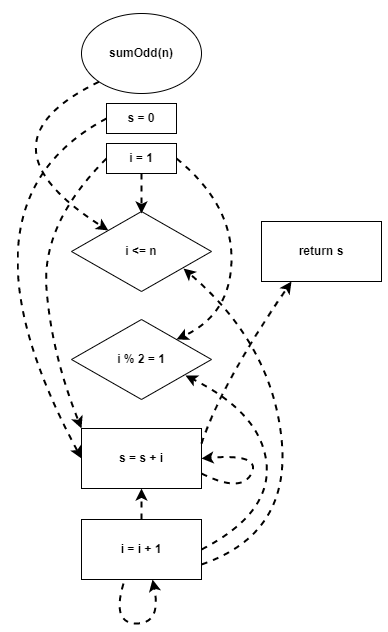
\includegraphics [scale=0.73] {my_folder/images/my/4}
	\caption{DDG}
	\label{fig:4}  
\end{figure}
\hfill \break
Исходя из всего вышесказанного, можно сделать вывод, что модели на основе CFG и DDG применимы для отдельных аспектов анализа кода, отражая лишь часть имеющихся зависимостей, и не обладают необходимой полнотой для всестороннего анализа исходного кода.
\newpage
\subsection{Граф зависимости программы} \label{ch1:subsec-title-abbr}
Граф зависимостей программы (Program Dependence Graph, PDG) – это объединенный граф потока данных и графа потока управления. Вершины PDG – это инструкции программы, а ребра – зависимости между ними. Есть две основных типов ребер: ребра выражающие зависимости по данным и ребра выражающие зависимости по управлению.
Граф зависимостей программы используется для:
\begin{itemize}
\item Оптимизации
\item Генерации кода
\item Анализа программ
\item Верификации
\item И т. п.
\end{itemize}

На рис. 1.5 изображен пример визуализации PDG.

\begin{figure}[h]
	\center
	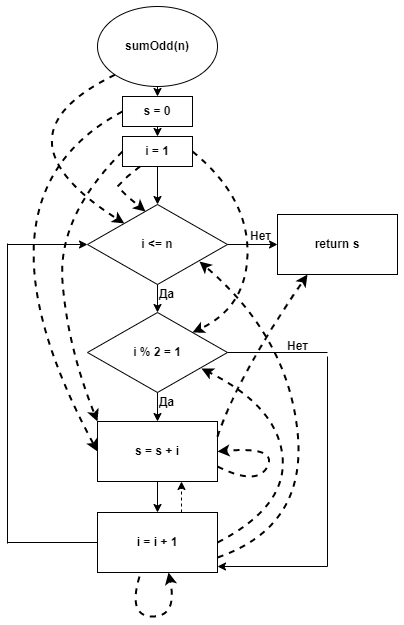
\includegraphics [scale=0.7] {my_folder/images/my/5}
	\caption{PDG}
	\label{fig:5}  
\end{figure}
\subsection{Абстрактный семантический граф} \label{ch1:subsec-title-abbr}
Абстрактный семантический граф (Abstract Semantic Graph, ASG) является расширением AST. ASG по сравнению с AST дополнен различными семантическим дугами, отображающими соответствующие семантические свойства программы и упрощающими навигацию по исходному коду. Данная модель обладает необходимой полнотой для всестороннего анализа исходного кода программы. Для ряда методов статического анализа целесообразно применение упрощенных видов ASG. рассматриваемых как отдельные модели. Подобные модели концентрируются на определенных семантических аспектах, за счет чего размерность и сложность моделей сокращаются.
На рис. 1.6 изображен пример визуализации ASG.

\begin{figure}[h]
	\center
	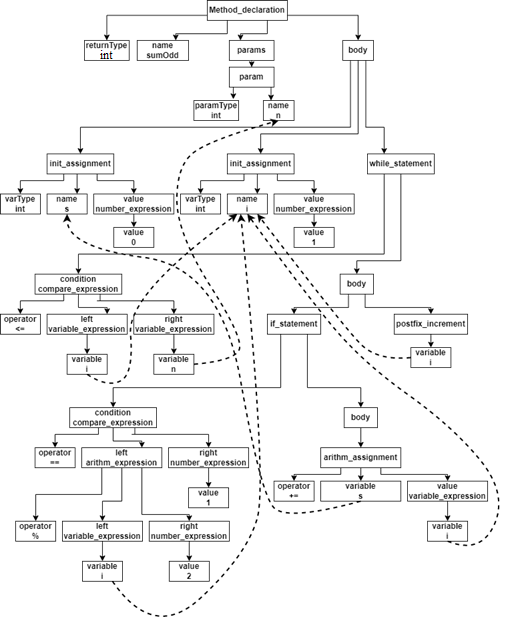
\includegraphics [scale=0.85] {my_folder/images/my/6}
	\caption{ASG}
	\label{fig:6}  
\end{figure}
\subsection{Представление на основе однократного статического присваивания} \label{ch1:subsec-title-abbr}
Представление на основе однократного статического присваивания (static single assignment, SSA) – это представление исходного кода программы, в котором:
\begin{itemize}
\item Каждой локальной переменной значение присваивается только один раз.
\item Вводится версионирование для локальных переменных, которые в исходном коде имеют неоднократные присваивания.
\item Для локальных переменных вводятся Фи-функции на выходе условных конструкций, объединяющие несколько ветвей программы и определяющие их окончательное значение
\item Циклы заменяются инструкциями ветвления и безусловных переходов
\end{itemize}
Данное представление может быть изображено в CFG-форме. На рис. 1.7 изображен пример визуализации SSA.
\begin{figure}[h]
	\center
	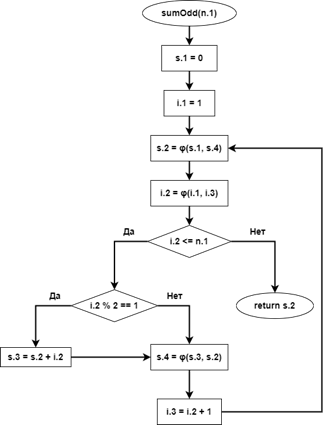
\includegraphics [scale=0.9] {my_folder/images/my/7}
	\caption{SSA}
	\label{fig:7}  
\end{figure}
\section{Выводы по главе} \label{ch1:sec3}
В данной главе были изучены методики исправления ошибок в программном коде и проведен анализ предметной области. Для каждой модели приведен теоретический обзор и представлен один из вариантов визуализации. Модельное представление программы призвано упростить и формализовать разработку алгоритмов статического анализа. При этом выбранное модельное представление должно обладать определенными свойствами, обеспечивающими эффективность и наглядность алгоритмов статического анализа.
\newpage